\documentclass{article}
\usepackage[T1]{fontenc}
\usepackage{lmodern}
\usepackage{graphicx}
\usepackage{amsmath,amssymb}
\usepackage[a4paper,margin=2cm]{geometry}
\usepackage[absolute,overlay]{textpos}
\setlength{\TPHorizModule}{1mm}
\setlength{\TPVertModule}{1mm}
\usepackage[indonesian]{babel}
\usepackage{hyperref}
\setlength{\emergencystretch}{2em}
% unit: Halaman 12

\begin{document}

% === Halaman 12 (llm) ===

Sumber asli dari dari dokumen FIPS-PUB

\vspace{118.80mm}

% deskripsi: Diagram alir proses penjadwalan kunci (key scheduling) dalam algoritma enkripsi, yang menunjukkan transformasi kunci 64-bit melalui Permuted Choice 1, pemisahan menjadi dua bagian (C dan D), pergeseran kiri (left shift) berulang, dan penggunaan Permuted Choice 2 untuk menghasilkan kunci sub-kunci K1 hingga K16.
% bbox normalisasi: [0.3040, 0.5300, 0.6800, 0.9300]
\begin{textblock*}{78.96mm}(63.84mm,157.41mm)
\noindent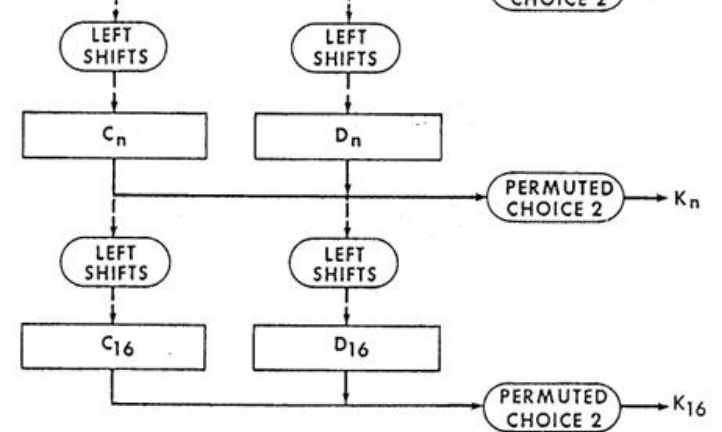
\includegraphics[width=78.96mm,height=118.80mm]{../../images/llm/page_012_img_01.png}%
\end{textblock*}

\end{document}
